\documentclass[a4paper]{article}


%%%%lualatex on
%\usepackage{luatextra}
\usepackage{fontspec}
%Ligatures={Contextual, Common, Historical, Rare, Discretionary}
%\setmainfont[Mapping=tex-text]{Linux Libertine O}

\usepackage{natbib}

\title{Notes model}
\author{Simon Carrignon}
\date{20-8-2015}

\begin{document}
\section{Model en mode Agent baseD}
After lot of experiment with different number of good and number of agent we can see that the number of goods impact a lot, and number of agent change, but not so much. It react not so much to ratio, but mor to number of goods

\begin{figure}[htp]
    \centering
    \begin{tabular}{cc}
	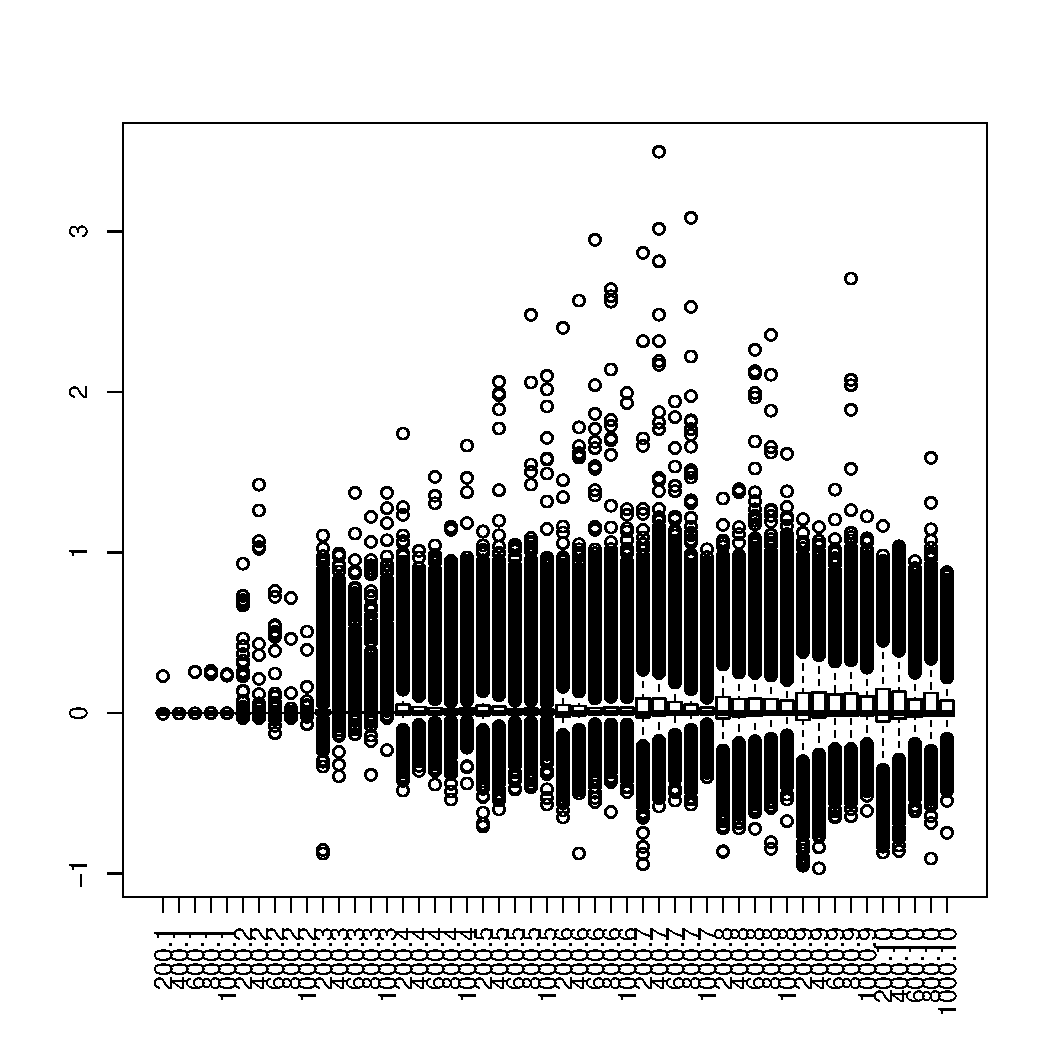
\includegraphics[width=3.5cm]{interactionNGoodNAgent.pdf}
	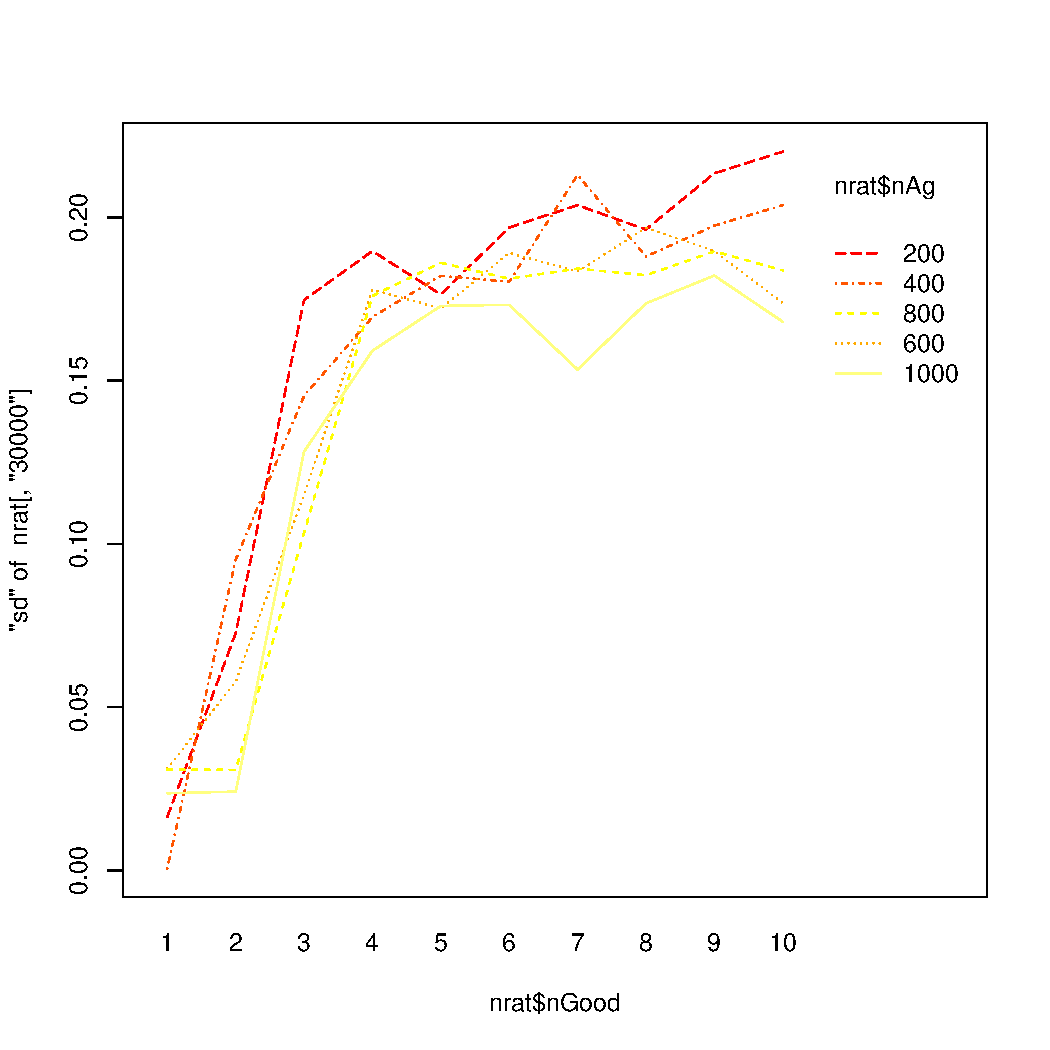
\includegraphics[width=3.5cm]{interactionNGoodNAgentSD.pdf}
    \end{tabular}
    \caption{Interaction between number of agent and number of good.}
\end{figure}

\section{New Mathematical stuff}

EQUATIOM: %TODO noter les equations!!!

Now the condition of acceptance of the 

test with $ngoods=3$ and $n_agents=500$ and $timeStep=30000$

\subsection{Score of the agents:}
\begin{figure}[htp]
    \centering
    \begin{tabular}{cc}
	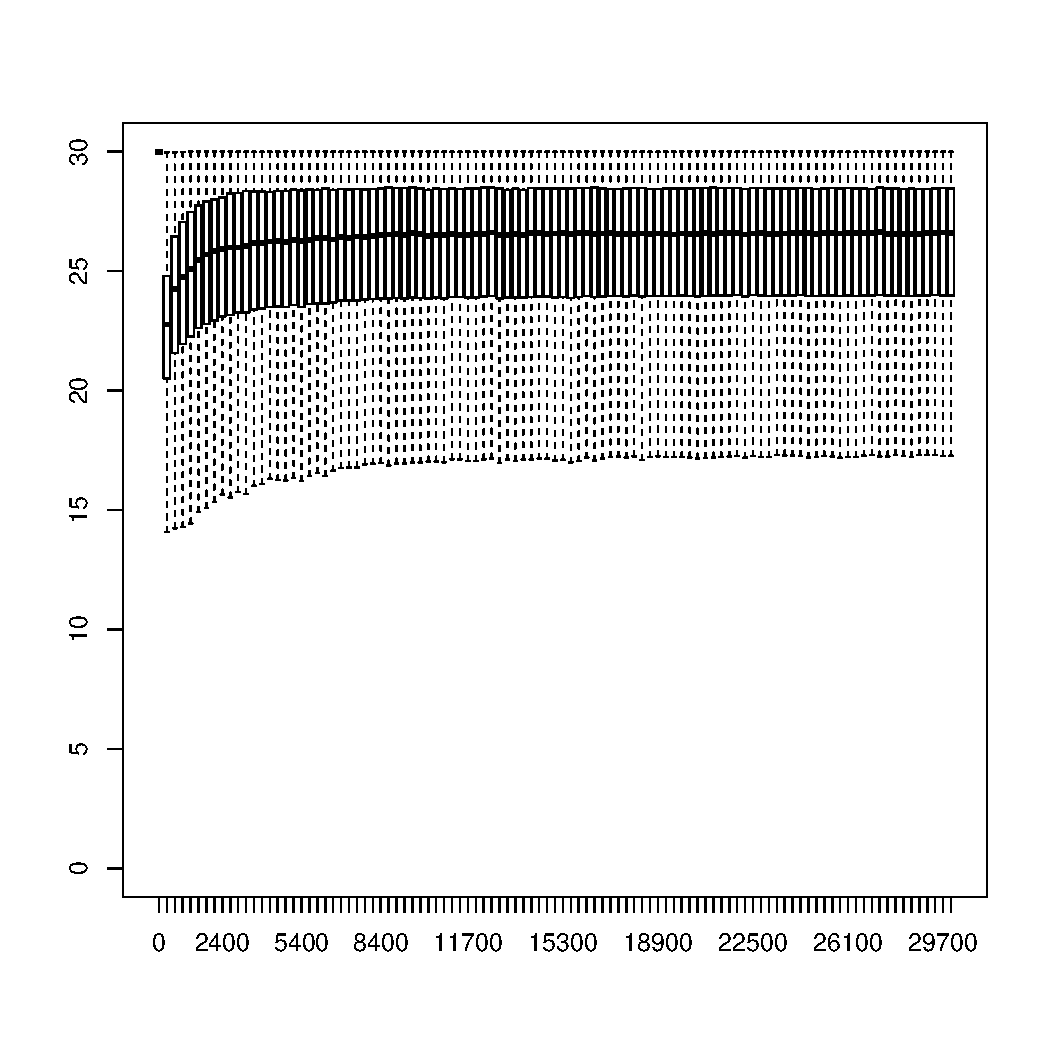
\includegraphics[width=5cm]{boxScoreTime.pdf}
	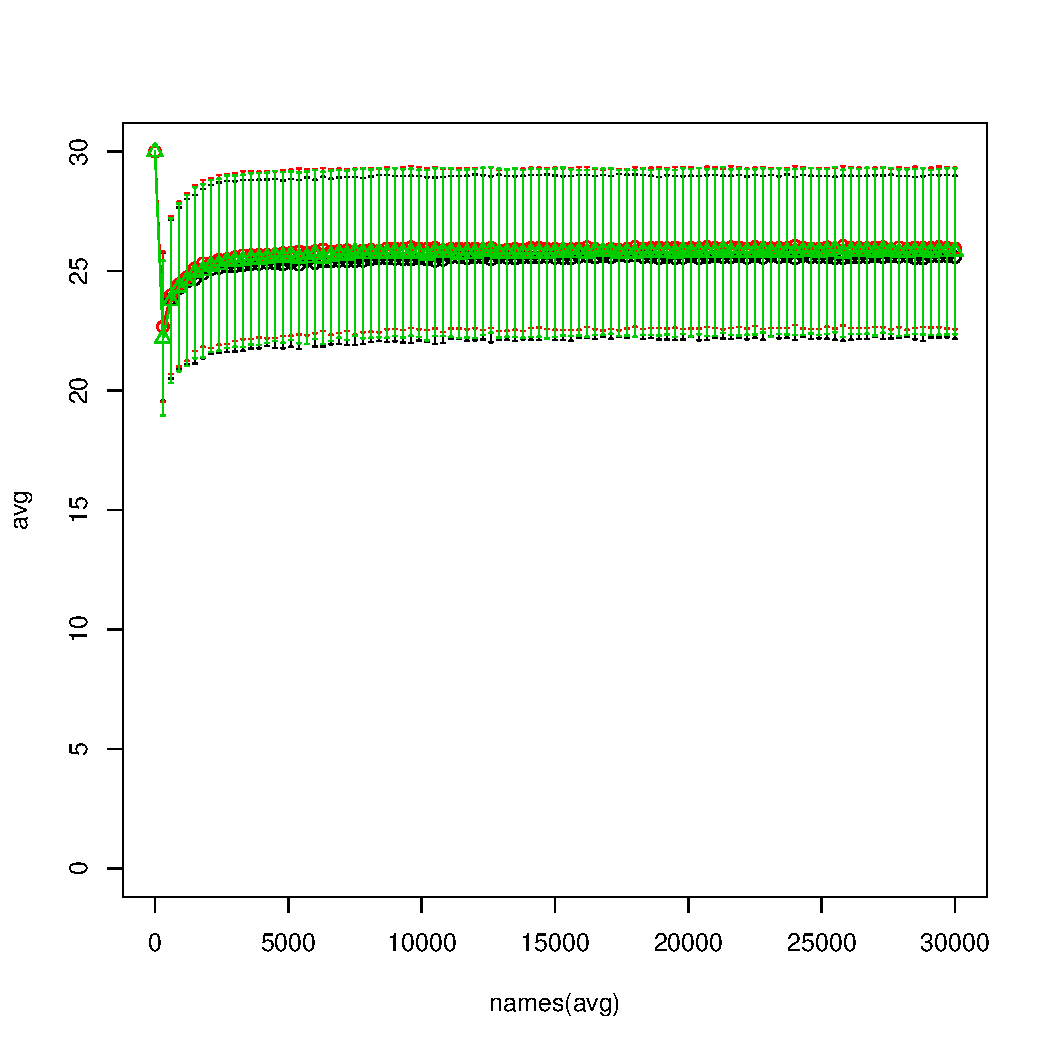
\includegraphics[width=5cm]{meanEachGroup.pdf}
    \end{tabular}
    \caption{Evolution of the score of the agent during the simulation.}
\end{figure}
\subsection{Difference of optimal price:}
(for the non produced price, I don't know for the produced one)
\begin{figure}[htp]
    \centering
    \begin{tabular}{cc}
	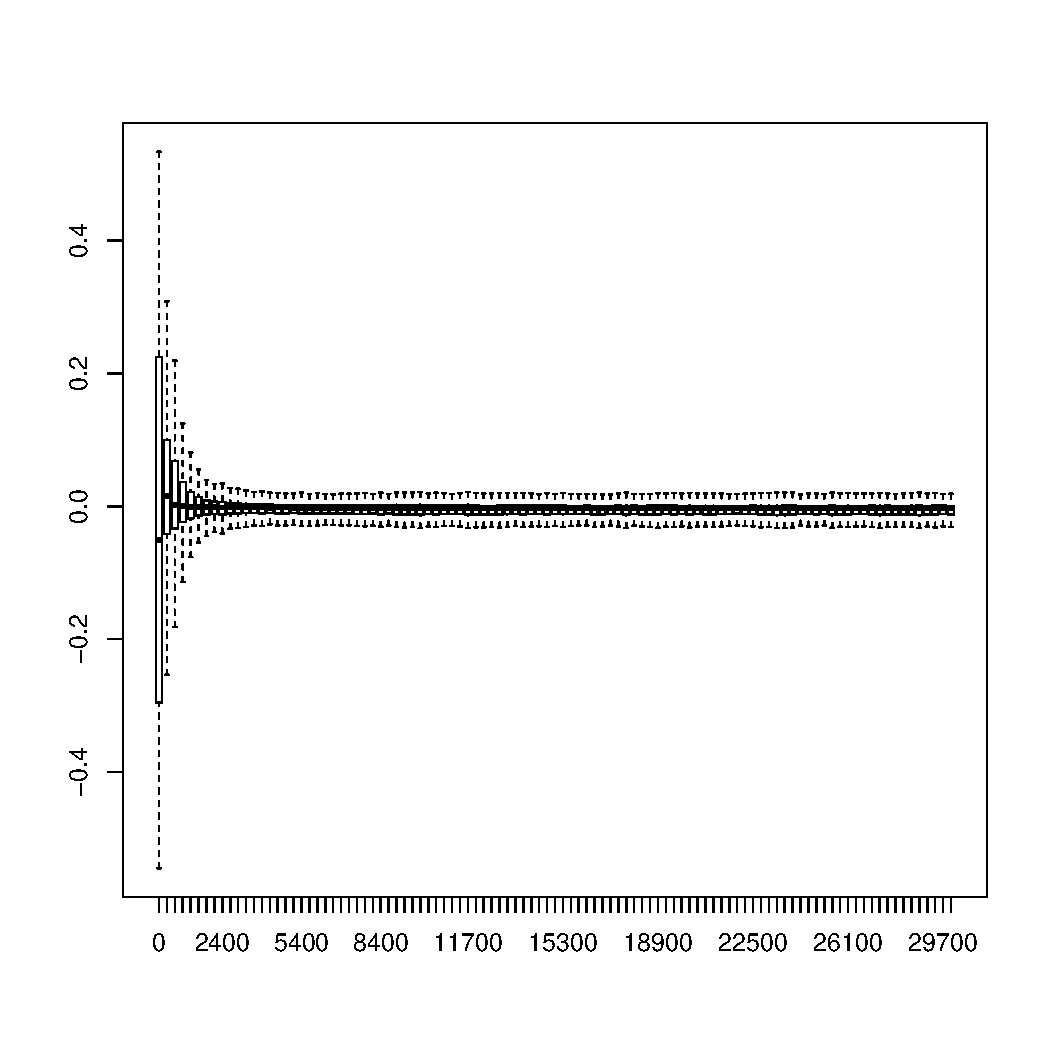
\includegraphics[width=3.5cm]{meanRatio.pdf}
    \end{tabular}
    \caption{Change of the price of the non produced good toward optimaproduced good toward optimal.}
\end{figure}

\end{document}
